  \documentclass[xcolor=table]{beamer}
\usepackage{beamerthemesplit}
\usepackage{wrapfig}
\usetheme{SPbGU}
\usepackage{pdfpages}
\usepackage{amsmath}
\usepackage{cmap} 
\usepackage[T2A]{fontenc} 
\usepackage[utf8]{inputenc}
\usepackage[english]{babel}
\usepackage{indentfirst}
\usepackage{amsmath}
\usepackage{tikz}
\usepackage{multirow}
\usepackage[noend]{algpseudocode}
\usepackage{algorithm}
\usepackage{algorithmicx}
\usepackage{fancyvrb}
\usetikzlibrary{shapes,arrows}
%usepackage{fancyvrb}
%\usepackage{minted}
%\usepackage{verbments}


\beamertemplatenavigationsymbolsempty

\title[Результаты группы за 2018 год]{Результаты группы за 2018 год}
\institute[СПбГУ]{
JetBrains Research, Programming Languages and Tools Lab  \\
Санкт-Петербургский Государственный Университет
}

\author[Семён Григорьев]{Семён Григорьев}

\date{15.12.2018}

\begin{document}
{
\begin{frame}[fragile]
  \begin{tabular}{p{2.0cm} p{7.5cm} p{1cm}}
   \begin{center}
      
\includegraphics[height=1.5cm]{pictures/jetbrainsResearch.pdf}
    \end{center}
    &
    \begin{center}
      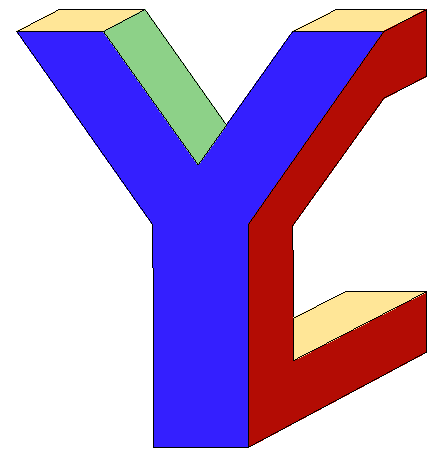
\includegraphics[height=1.5cm]{pictures/YC_logo.pdf}
    \end{center}
    &
    \begin{center}
      
\includegraphics[height=1.5cm]{pictures/SPbGU_Logo.png}
    \end{center} 
  \end{tabular}
  \titlepage
\end{frame}
}


\begin{frame}[fragile]
  \transwipe[direction=90]
  \frametitle{Области интересов}
\begin{itemize}
      \item Теория формальных языков
      \item Алгоритмы синтаксического анализа
      \item Применение теории формальных языков и синтаксического анализа для решения прикладных задач
      \begin{itemize}
        \item Статический анализ кода
        \item Анализ графовых баз даных
        \item Биоинформатика
        \item \textit{Поиск новых областей}
      \end{itemize}

\end{itemize}

\end{frame}

\begin{frame}[fragile]
  \transwipe[direction=90]
  \frametitle{Научные конференции}
\begin{itemize}

      \item \textbf{ICFP-2018}
      \begin{itemize}
        \item \emph{Екатерина Вербицкая}, Илья Кириллов, Илья Ножкин, Семён Григорьев. Parser Combinators for Context-Free Path Querying (Scala~simposium)
        \item \emph{Семён Григорьев}, Кирилл Смиренко. F\# OpenCL C Type Provider (TyDe)
      \end{itemize}

      \item \textbf{SIGMOD-2018} (доклад + постер)
      \begin{itemize}
        \item \emph{Екатерина Вербицкая}, Рустам Азимов, Семён Григорьев. Context-Free Path Querying by Matrix Multiplication (GRADES-NDA)
      \end{itemize}
      
      \item \textbf{Google Compiler and Programming Language Summit} (постер)
      \begin{itemize}
        \item \emph{Екатерина Вербицкая}. Graph Querying by Parsing 
      \end{itemize}

      \item \textbf{BIATA-2018} (постер)
      \begin{itemize}
         \item \emph{Семён Григорьев}, Полина Лунина. 16s rRNA Detection by Using Neural Networks 
      \end{itemize}
      
      \item \textbf{Современные технологии в теории и практике программирования}
      \begin{itemize}
         \item С.А. Варивода, А.Д. Милакин, А.А.~Солдатенков (ЛЭТИ), С.В.~Григорьев. Контекстно чувствительный анализ алиасов
      \end{itemize}

\end{itemize}
\end{frame}
 
\begin{frame}[fragile]
  \transwipe[direction=90]
  \frametitle{Доклады}
\begin{itemize}

      \item \textbf{JetBrains Internal Conference-2018}
      \begin{itemize}
        \item Formal Languages Theory is not Only About Parsing
      \end{itemize}

      \item Cеминар по алгоритмической математике (ЛЭТИ, \url{http://pozdnkov.vm2-leti.spb.ru/iniciativy/proekty/seminar-po-algoritmiceskoj-matematike})

      \item Встречи тематических групп (FProg, IT Global Meetup)

\end{itemize}
\end{frame}


\begin{frame}[fragile]
  \transwipe[direction=90]
  \frametitle{Публикации}
\begin{itemize}
      \item Материалы конференций
        \begin{itemize}
          \item \textbf{ICFP, SIGMOD} --- ACM
          \item Остальное --- сборники материалов конференций
        \end{itemize}
      \item Азимов Р. Ш., Григорьев С. В. Синтаксический анализ графов с использованием конъюнктивных грамматик // Труды института системного программирования РАН. – 2018. (ВАК)
\end{itemize}
\end{frame}

\begin{frame}[fragile]
  \transwipe[direction=90]
  \frametitle{Сотрудничество}
\begin{itemize}
      \item Грант РНФ под руководством Александра Охотина
      \item INRIA LINKS (\url{https://team.inria.fr/links/})
      \begin{itemize}
         \item Стажировка Рустама Азимова (сентябрь-ноябрь 2018)
         \item Планируется поездка Семёна Григорьева в апреле 2019
      \end{itemize}
      \item Применение теории формальных языков для межпроцедурного анализа в рамках проекта ReSharper (в процессе)
      \item Применение теории формальных языков для получения информации о типах в Ruby (в процессе)
      \begin{itemize}
         \item Команда RubyMine
         \item Sebastian Erdweg, Programming Languages Research Group, TU Delft
      \end{itemize}
      
\end{itemize}
\end{frame}

\begin{frame}[fragile]
  \transwipe[direction=90]
  \frametitle{Сотрудничество}
\begin{itemize}
      \item Phillip Bradford, University of Connecticut, Stamford, субкубический~алгоритм поиска путей с КС ограничениями
      \item Carlo Sartiani, Università degli Studi della Basilicata: Potenza, Basilicata, применение производных для распределённого выполнения КС запросов
      \item Witold Dyrka, Institute of Biomedical Engineering and Instrumentation, Wroclaw University of Technology, применение~синтаксического анализа в биоинформатике
      
\end{itemize}
\end{frame}


\begin{frame}[fragile]
  \transwipe[direction=90]
  \frametitle{Образовательная деятельность}
\begin{itemize}
      \item Курс (лекции/семинары) по теории формальных языков 
%      \begin{itemize}
%         \item Математико-Механический факультет СПбГУ
%         \item ЛЭТИ
%         \item АУ
%      \end{itemize}
      \item Курс по теории графов на математико-механическом факультете СПбГУ
      \item Семинар по теории формальных языков
      \item Руководство курсовыми, ВКР, магистерскими, семестровыми проектами и т.д.
\end{itemize}
\end{frame}

\begin{frame}[fragile]
  \transwipe[direction=90]
  \frametitle{Планируемые публикации}
\begin{itemize}
      \item Semyon Grigorev, Polina Lunina. The Composition of Dense Neural Networks and Formal Grammars for Secondary Structure Analysis. Подана на BIOINFORMATICS-2019
      \item Rustam Azimov, Semyn Grigorev. Path Querying with Conjunctive Grammars by Matrix Multiplication. Подана на LATA-2019
      \item Sergey Bozhko, Leyla Khatbullina, Semyon Grigorev. Bar-Hillel~Theorem Mechanization in Coq. Подготовлена
\end{itemize}
\end{frame}

\begin{frame}[fragile]
  \transwipe[direction=90]
  \frametitle{Ведущиеся работы}
\begin{itemize}
      \item Логарифмическая схема для поиска путей с КС ограничениями. Екатерина Шеметова, Семён Григорьев, Александр Охотин
      \item Субкубический алгоритм. Екатерина Шеметова, Рустам Азимов, Семён Григорьев, Phillip Bradford
      \item Улучшение матричного алгоритма синтаксического анализа. Юлия Сусанина, Семён Григорьев, Александр Охотин
      \item Применение синтаксического анализа для обработки биологических последовательностей. Полина Лунина, Семён~Григорьев
      \item Построение группы по формальному языку: попытка построить алгоритм по статье Isoperimetric and Isodiametric Functions of Groups, Mark V. Sapir, Jean-Camille Birget and Eliyahu Rips
\end{itemize}
\end{frame}


\begin{frame}[fragile]
  \transwipe[direction=90]
  \frametitle{Планируемые работы}
\begin{itemize}
      \item Разработка и исследование алгоритмов поиска путей с ограничениями в виде формальных грамматик
      \begin{itemize}
        \item Конъюнктивные граммтики на основе BRNGLR
        \item Производные
        \item Распределённые алгоритмы
      \end{itemize}
      \item Исследование связи алгебры с теорией формальных языков (в~широком смысле) 
\end{itemize}
\end{frame}

\begin{frame}[fragile]
  \transwipe[direction=90]
  \frametitle{Направления}
\begin{itemize}
      \item Публикации на тематических конференциях (DLT, LATA, SIGMOD)
      \item Переход к более фундаментальным задачам
      \item Более активное сотрудичество с коллегами
\end{itemize}
\end{frame}

\end{document}
